\documentclass[11pt]{article}

\usepackage[margin=1in]{geometry}
\usepackage{amsmath,amssymb,amsthm,mathtools}
\usepackage{bm}
\usepackage{graphicx}
\usepackage{booktabs}
\usepackage{multirow}
\usepackage[round]{natbib}
\usepackage{xcolor}
\usepackage[colorlinks=true,linkcolor=blue!60!black,citecolor=blue!60!black,urlcolor=blue!60!black]{hyperref}
\usepackage{microtype}
\usepackage{caption}
\captionsetup{font=small,labelfont=bf}

\newtheorem{theorem}{Theorem}
\newtheorem{lemma}{Lemma}
\newtheorem{corollary}{Corollary}
\newtheorem{definition}{Definition}
\newtheorem{remark}{Remark}

\newcommand{\R}{\mathbb{R}}
\newcommand{\silu}{\mathrm{SiLU}}
\newcommand{\T}{^{\top}}
\DeclareMathOperator{\rank}{rank}
\DeclareMathOperator{\diag}{diag}

\title{How Much Tensor Structure Should a Transformer FFN Have?\\
\large Routed Block-CP Feedforward Networks Between SwiGLU and Dense Tucker}

\author{Aniket Deshpande\\
University of Illinois Urbana-Champaign\\
\texttt{aniket4@illinois.edu}}

\date{June 2026}

\begin{document}
\maketitle

\begin{abstract}
Transformer feedforward networks hold most of a language model's parameters, but
their multiplicative interactions lack the structural vocabulary that makes attention
analyzable. We start from an exact observation: a SwiGLU block is a \emph{routed CP
tensor model} --- each hidden channel contributes a fixed rank-one interaction atom
$u_j \otimes w_j \otimes g_j$, routed by an input-dependent sigmoid coefficient. The
superdiagonal latent core this implies is both what atomizes the layer and what
restricts every route to a single rank-one interaction. Rather than replacing it with
an arbitrary dense Tucker core, we study the family that interpolates between the
two: LL1 (block-term) feedforward networks, in which one gate routes a rank-$L$ block
of interactions, so that the per-route rank --- exactly the quantity priced by an
aligned-width separation theorem --- becomes a hyperparameter, and, at fixed
parameters, routing diversity is traded for interaction atoms. In controlled
teacher--student recovery, routes and per-route rank are independently binding:
students recover a routed tensor map to machine precision exactly when both suffice,
and the nominally most expressive dense core loses every matched-budget comparison.
On real pretrained FFN layers (Qwen2.5-0.5B), LL1 students with $L\approx4$--$8$
compress the layer's function better than rank-one atoms in every layer and budget
tested, and far better than a dense core. Trained from scratch at matched parameters
and FLOPs (52.5M parameters, 100M tokens, 3 seeds), SwiGLU, LL1($L{=}4$), and dense
Tucker tie on validation loss --- while LL1 trains 5--7\% faster than SwiGLU and
$2.1\times$ faster than Tucker, and an unconstrained Tucker core spontaneously learns
per-route stable rank $\approx 4$, the same value at which LL1's blocks saturate and
the distillation optimum sits. Interpretability proxies are a deliberate negative:
no architecture routes sparsely, and LL1's learned blocks recur across seeds no
better than chance. Our results suggest that the right amount of tensor structure in
a transformer FFN is a measurable quantity --- about rank four per route at this
scale --- and that structured block-CP parameterizations deliver it at zero loss cost,
but that architectural structure alone does not purchase mechanistic
interpretability.
\end{abstract}

\section{Introduction}

Attention has accumulated a rich structural vocabulary --- heads, QK/OV circuits,
induction patterns \citep{elhage2021mathematical,olsson2022context} --- that makes it
the best-understood component of transformers. The feedforward network, which holds
the majority of parameters in modern architectures
\citep{vaswani2017attention,shazeer2020glu}, has no comparable account: its
multiplicative gating creates feature interactions that are hard to trace through
weights, and most interpretability progress on MLPs has come from analyzing
activations rather than the architecture itself
\citep{bricken2023monosemanticity,dunefsky2024transcoders}.

The starting point of this paper is that for SwiGLU --- the dominant FFN variant ---
an exact architectural account already exists, hidden in plain sight. Because
$\silu(z) = z\,\sigma(z)$, each SwiGLU channel is a rank-one bilinear interaction
between two learned directions, scaled by a sigmoid gate: the layer is, exactly and
pointwise in its input, a CP decomposition of a third-order interaction tensor with
fixed factors and input-dependent routing weights (\S\ref{sec:routedcp}). Each hidden
index contributes one \emph{atom} (what interaction is available) and one
\emph{route} (when it is used). This is the gated counterpart of the bilinear-MLP
observation of \citet{pearce2025bilinear}, who showed that GLUs \emph{without} the
element-wise nonlinearity are third-order tensors amenable to weight-based analysis.

The CP structure cuts both ways. Read as a Tucker decomposition, SwiGLU's latent core
is superdiagonal: the $j$-th main feature interacts only with the $j$-th gate. This
restriction is what makes the decomposition atomized and essentially unique
\citep{kruskal1977three} --- ``CPD gives a sparse core for free'' --- but it also
means one route controls exactly one rank-one interaction. An earlier draft of this
project proposed the obvious mathematical relaxation, a dense learned core (a
Tucker-FFN), and proved a separation theorem: simulating a Tucker block with aligned
SwiGLU units costs $\sum_j \rank V_j$ units, where $V_j$ is the interaction matrix
routed by gate $j$ --- generically $k^2$ versus $O(k)$ latent dimensions. We now
believe the dense core is the wrong conclusion to draw from that theorem. A dense
core is gauge-non-identifiable (its latent directions carry no intrinsic meaning),
concentrates $\sim$90\% of the block's parameters in interactions, and --- as our
experiments show --- is dominated in practice. The right reading of the theorem is
that \emph{the per-route rank $\rank V_j$ is the priced quantity}, and the
constructive half of its proof is itself an architecture: realize each $V_j$ as $L$
rank-one atoms sharing one gate.

That architecture is the LL1 (multilinear rank-$(L,L,1)$ block-term) decomposition
\citep{delathauwer2008blockterm} applied to the FFN's interaction tensor, with the
gate mode as the rank-one mode (\S\ref{sec:ll1}). It nests SwiGLU exactly at $L{=}1$
and block-sparse Tucker in general, and it makes the comparison crisp at a fixed
parameter budget: an LL1 block buys $\tfrac{3L}{2L+1}\times$ more interaction atoms
than SwiGLU at the price of $\tfrac{3}{2L+1}\times$ fewer independent routes.
\emph{How much rank should a route control?} becomes an empirical question with a
dial.

We answer it with four experiments at strictly matched parameters and FLOPs:
synthetic teacher--student recovery where the true structure is known
(\S\ref{sec:synthetic}); compression of real pretrained FFN layers
(\S\ref{sec:distill}); from-scratch language-model training (\S\ref{sec:lm}) with
measured throughput; and interpretability proxies plus an induction-circuit pilot
(\S\ref{sec:interp}--\ref{sec:induction}).

Our contributions:
\begin{enumerate}
\item \textbf{Framing (exact):} SwiGLU as a routed CP tensor field; the LL1 FFN as
  the rank-controlled family between routed CP and dense Tucker, nesting both; the
  route/atom budget identity; and the aligned-width theorem re-read as pricing
  per-route rank (Appendix~\ref{app:theorem}).
\item \textbf{Recovery (synthetic):} at fixed budget, routes and per-route rank bind
  independently --- error is minimized exactly at the teacher's block rank, with
  machine-precision recovery if and only if structure matches, and the dense core
  loses every cross-class comparison.
\item \textbf{Real FFN maps:} distilling Qwen2.5-0.5B layers, LL1 with
  $L\approx4$--$8$ beats rank-one atoms in all nine layer$\times$budget cells
  ($\sim$30$\times$ seed noise) and the dense core loses by 35--130\%.
\item \textbf{End-to-end:} at 52.5M parameters / 100M tokens (3 seeds), LL1($L{=}4$),
  SwiGLU, and Tucker tie on loss; LL1 is 5--7\% faster than SwiGLU and $2.1\times$
  faster than Tucker; and the unconstrained Tucker core spontaneously learns
  per-route stable rank $\approx 4$ --- the value LL1 hard-codes.
\item \textbf{Interpretability (negative):} measured proxies — routing diffuseness,
  top-$k$ decomposability, ablation locality, cross-seed factor recurrence — do not
  support the hypothesis that block structure improves mechanistic accessibility;
  LL1's blocks recur across seeds at chance. The induction pilot shows no effect of
  FFN structure on circuit emergence, with a single-seed observation of an
  alternative dense-core copying circuit.
\end{enumerate}

\section{The routed tensor view of gated FFNs}
\label{sec:theory}

\paragraph{Setup.}
At a fixed token position, let $x \in \R^d$ be the residual-stream vector entering the
feedforward block. The SwiGLU FFN \citep{shazeer2020glu} computes
\begin{equation}
\label{eq:swiglu}
y = U\T h, \qquad h = (W\T x) \odot \silu(G\T x),
\end{equation}
with $W, G \in \R^{d\times m}$ and $U \in \R^{m \times d}$. Writing $w_j, g_j$ for the
$j$-th columns of $W, G$ and $u_j$ for the $j$-th column of $U\T$, the $j$-th hidden
coordinate is $h_j(x) = (w_j\T x)\,\silu(g_j\T x)$.

\subsection{SwiGLU is an exactly routed CP tensor field}
\label{sec:routedcp}

Each SwiGLU channel multiplies two scalar projections of the residual stream. The SiLU
nonlinearity factorizes exactly, $\silu(z) = z\,\sigma(z)$ with
$\sigma(z) = (1+e^{-z})^{-1}$, so
\begin{equation}
\label{eq:factorized}
h_j(x) \;=\; \underbrace{(w_j\T x)(g_j\T x)}_{\text{rank-one bilinear interaction}}
\cdot \underbrace{\sigma(g_j\T x)}_{\alpha_j(x)\,\in\,(0,1)} .
\end{equation}
Defining the input-dependent interaction tensor $A(x) \in \R^{d\times d\times d}$ by
$y_o = \sum_{a,b} A_{oab}(x)\, x_a x_b$, substituting \eqref{eq:factorized} into
\eqref{eq:swiglu} gives
\begin{equation}
\label{eq:cp}
A(x) \;=\; \sum_{j=1}^{m} \alpha_j(x)\; u_j \otimes w_j \otimes g_j ,
\qquad \alpha_j(x) = \sigma(g_j\T x).
\end{equation}
This is a canonical polyadic (CP) decomposition \citep{kolda2009tensor} of $A(x)$ with
\emph{shared, input-independent factors} and \emph{input-dependent routing weights}
$\alpha_j(x)$. The decomposition is exact and holds pointwise in $x$; no approximation
is involved. We call $u_j \otimes w_j \otimes g_j$ the $j$-th \emph{interaction atom}
(what interaction is available) and $\alpha_j(x)$ its \emph{route} (when it is used).
The bilinear $\alpha\equiv 1$ limit of this picture is the bilinear MLP analyzed by
\citet{pearce2025bilinear}; the routed form keeps the gate inside the structural
description rather than discarding it.

Viewed as a Tucker decomposition with latent dimensions $r=s=m$ and factor matrices
$(P,Q,R) = (W, G, U\T)$, the CP form \eqref{eq:cp} corresponds to a
\emph{superdiagonal core}: $C_{oij} = \delta_{oi}\delta_{ij}$. This restriction cuts
both ways. It atomizes the layer --- every hidden index is one (atom, route) pair, and
CP decompositions are essentially unique under mild conditions
\citep{kruskal1977three}, so the atoms are identifiable objects. But it also means one
route controls exactly one rank-one interaction: feature $w_i$ never interacts with
gate $g_j$ for $i \ne j$.

\subsection{Dense Tucker and the per-route interaction matrix}
\label{sec:tucker}

The unconstrained relaxation drops the superdiagonal restriction. A
\emph{Tucker-core FFN} with latent projections $P, Q \in \R^{d\times r}$, output basis
$R \in \R^{d \times s}$, and learned core $C \in \R^{s\times r\times r}$ computes
$p = P\T x$, $q = Q\T x$,
\begin{equation}
\label{eq:tuckerffn}
z_o = \sum_{i,j=1}^{r} C_{oij}\, p_i\, \silu(q_j), \qquad y = Rz .
\end{equation}
Grouping by gate index exposes the structure this paper is about:
\begin{equation}
\label{eq:vj}
y(x) = \sum_{j=1}^{r} V_j\, p \; \silu(q_j), \qquad V_j := R\,C^{(j)} \in \R^{d\times r},
\quad C^{(j)}_{oi} = C_{oij}.
\end{equation}
Each latent gate $q_j$ routes a \emph{matrix} $V_j$ of output-by-main interactions.
SwiGLU is the corner case $\rank V_j = 1$ for all $j$; a generic Tucker core has
$\rank V_j = \min(r,s)$.

Two properties make the dense core suspicious as an interpretability target. First,
\emph{gauge freedom}: for any invertible $M \in \R^{r\times r}$, replacing $P \mapsto
P M^{-\top}$ and $C^{(j)} \mapsto C^{(j)} M$ for all $j$ leaves the function
unchanged, so individual latent directions $p_i$ and individual core entries carry no
intrinsic meaning --- only the gate directions $Q_{:j}$ and the subspaces
$\mathrm{range}(V_j)$ are well defined. Second, the core costs $s r^2$ parameters; at
the configurations we study it absorbs over $90\%$ of the block's budget.

\paragraph{The aligned-width theorem, reinterpreted.}
Prior work on this codebase proved an exact separation: if $[P\;Q]$ has full column
rank, an \emph{aligned} SwiGLU (units restricted to main vectors in $\mathrm{span}(P)$
and gate vectors from the columns of $Q$) that exactly realizes \eqref{eq:vj} must have
width $m \ge \sum_j \rank V_j$, and a rank decomposition of each $V_j$ attains the
bound (Appendix~\ref{app:theorem}). Generically this is $r\min(r,s)$, i.e.\ $k^2$ in
the balanced case --- the result that originally motivated dense Tucker as
``$k\times$ cheaper than SwiGLU.'' The reading we adopt here is different: \emph{the
theorem says the operative variable is the per-route rank $\rank V_j$}, not the
presence of a dense core. The constructive half of the proof --- realize each $V_j$ as
a sum of $\rank V_j$ rank-one terms sharing the same gate --- is itself an
architecture. That architecture is the subject of this paper.

\subsection{LL1/block-CP: one route, one rank-$L$ block}
\label{sec:ll1}

A third-order tensor admits a \emph{decomposition in multilinear rank-$(L,L,1)$ terms}
(LL1; a structured block-term decomposition) if it can be written
$T = \sum_{b=1}^{B} (A_b B_b\T) \otimes c_b$: each term is rank-$L$ in two modes and
rank-one in the third \citep{delathauwer2008blockterm,vervliet2016tensorlab}. Taking
the \emph{gate mode} as the rank-one mode yields the FFN we study. The
\textbf{LL1 FFN} with $B$ blocks of rank $L$ has, per block, a gate direction
$g_b \in \R^d$, a main factor $A_b \in \R^{d\times L}$, and an output factor
$U_b \in \R^{d \times L}$:
\begin{equation}
\label{eq:ll1}
y(x) \;=\; \sum_{b=1}^{B} U_b \big(A_b\T x\big)\, \silu(g_b\T x).
\end{equation}
Expanding into atoms, $y(x) = \sum_b \sum_{l=1}^{L} u_{b,l} (a_{b,l}\T x)\,
\silu(g_b\T x)$: \emph{grouped CP}, $L$ rank-one atoms sharing one route. The
interaction tensor is the routed LL1 tensor
$A(x) = \sum_b \alpha_b(x)\, (U_b A_b\T) \otimes g_b$, and the per-route matrix is
$V_b = U_b A_b\T$ with $\rank V_b \le L$ \emph{by construction}. The aligned-width
theorem's control variable has become a hyperparameter.

The family nests both endpoints exactly. At $L=1$, $B=m$, \eqref{eq:ll1} \emph{is}
SwiGLU (verified to machine precision in our implementation); a single block with
$L = r$ is a (one-gate) dense slice; and an LL1 FFN equals a Tucker FFN whose core is
block-superdiagonal. LL1 decompositions also retain essential-uniqueness guarantees
under mild conditions \citep{delathauwer2008blockterm,delathauwer2011blockterm},
unlike the gauge-free dense core.

\paragraph{What the parameter budget buys.}
The comparison that matters is at matched parameters:
\begin{equation}
\label{eq:params}
N_{\text{SwiGLU}} = 3dm, \qquad
N_{\text{LL1}} = dB(2L+1), \qquad
N_{\text{Tucker}} = d(2r+s) + sr^2 .
\end{equation}
At a fixed budget $N$, SwiGLU affords $m = N/3d$ atoms, each with a private route; LL1
affords $BL = \tfrac{3L}{2L+1}\cdot\tfrac{N}{3d}$ atoms --- up to $1.5\times$ more ---
but only $B = \tfrac{3}{2L+1}\cdot\tfrac{N}{3d}$ routes. \emph{LL1 trades routing
diversity for interaction atoms.} An equivalent statement: an LL1$(B,L)$ block is
exactly a width-$BL$ SwiGLU whose gate vectors are tied in groups of $L$. Which side
of the trade wins is an empirical question about what trained FFNs actually need, and
it is the question our experiments are designed to answer. A prior observation
sharpens the stakes: in a dense Tucker LM trained from scratch, the learned per-gate
stable rank $\|V_j\|_F^2/\|V_j\|_{\mathrm{op}}^2$ concentrates around $4$ --- far
below the generic value $r$, far above the SwiGLU value $1$. The trained dense core
already behaves like an LL1 model; LL1 makes that behavior an explicit and cheaper
parameterization (with essential-uniqueness guarantees at the decomposition level,
though \S\ref{sec:interp} shows these do not translate into cross-seed stability of
learned factors).

\begin{figure}[t]
\centering

\includegraphics[width=\textwidth]{figures/fig1_ladder.pdf}
\caption{The architecture family, indexed by per-route rank. \textbf{A)} A SwiGLU
channel: two projections of the residual stream are multiplied and scaled by the
route $\alpha_j(x) = \sigma(g_j\T x)$; the channel contributes the rank-one atom
$u_j \otimes w_j \otimes g_j$. \textbf{B)} An LL1 block: one route scales a rank-$L$
bundle $V_b = U_b A_b\T$ of interactions ($L$ atoms sharing a gate). \textbf{C)}
A dense Tucker core couples every latent main feature to every latent gate; each of
its $r$ routes carries a generically full-rank $V_j$, and the latent basis is not
identifiable. \textbf{D)} At a fixed parameter budget the family trades routes
against per-route rank (rectangles drawn to scale for the LM configuration of
Table~\ref{tab:configs}; area $\propto$ interaction atoms).}
\label{fig:ladder}
\end{figure}

\section{Experiments}
\label{sec:experiments}

All architectures are compared at matched parameter and FLOP budgets
(Table~\ref{tab:configs}; budgets match to $\pm 0.2\%$), with identical optimizers,
schedules, and data. Code, configurations, and per-seed results accompany the paper;
full hyperparameters are in Appendix~\ref{app:details}.

\begin{table}[t]
\centering
\small
\begin{tabular}{lccccc}
\toprule
architecture & config & routes & per-route rank & atoms ($\sum_j \rank V_j$) & FFN params/layer \\
\midrule
SwiGLU & $m{=}1493$ & 1493 & 1 & 1493 & 2{,}293{,}248 \\
LL1 $L{=}2$ & $B{=}896$ & 896 & 2 & 1792 & 2{,}293{,}760 \\
LL1 $L{=}4$ & $B{=}498$ & 498 & 4 & 1992 & 2{,}294{,}784 \\
LL1 $L{=}8$ & $B{=}263$ & 263 & 8 & 2104 & 2{,}289{,}152 \\
LL1 $L{=}16$ & $B{=}136$ & 136 & 16 & 2176 & 2{,}297{,}856 \\
dense Tucker & $r{=}s{=}128$ & 128 & 128 & 16384$^*$ & 2{,}293{,}760 \\
\bottomrule
\end{tabular}
\caption{Matched-budget configurations at $d=512$ (the LM setting of
\S\ref{sec:lm}). LL1 converts routing diversity into interaction atoms at fixed
budget. $^*$Tucker's atom count is the aligned-SwiGLU width its generic core would
require (Theorem~\ref{thm:bottleneck}); its parameters are concentrated in the core
($sr^2 = 2.10$M of $2.29$M).}
\label{tab:configs}
\end{table}

\subsection{Synthetic teacher--student recovery: structure must match, in both directions}
\label{sec:synthetic}

\textbf{Question.} Is per-route rank a real capacity dial — does a student recover a
routed tensor map if and only if its routes and per-route ranks suffice?

\textbf{Setup.} Teachers at $d=64$ with unit-variance outputs: a CP teacher (32
rank-one routed atoms), an LL1 teacher ($B^*{=}16$ blocks of rank $L^*{=}4$, i.e.\ 64
atoms on 16 routes), and a dense Tucker teacher ($r{=}s{=}16$, generic full-rank
slices). Students of every family are trained on Gaussian inputs by MSE at a fixed
9{,}216-parameter budget, 3 seeds; we report validation MSE relative to output
variance (best of 3, capacity reading; bands span seeds).

\textbf{Result.} Figure~\ref{fig:synthetic} (left to right): on the CP teacher,
$L{=}1$ students recover it (rel.\ MSE $\sim 10^{-4}$) and error rises monotonically
with $L$ (gate-tying starves routes: an $L{=}16$ student has only $B{=}4$ routes for a
32-route teacher). On the LL1 teacher the error minimum sits exactly at $L=L^*=4$
(machine precision, $2\times10^{-13}$, 2/3 seeds), with failure on both sides:
$L{<}4$ students lack atoms ($48, 58 < 64 = \sum_b \rank V_b$), the $L{=}8$ student
lacks routes ($8 < 16$). On the Tucker teacher only the Tucker student succeeds
($1.1\times10^{-10}$); every CP/LL1 student plateaus at rel.\ MSE $\ge 0.2$.

\textbf{Interpretation.} Routes and per-route rank are \emph{independently binding}
resources at fixed budget, exactly as the counting argument predicts, and each family
attains machine-precision recovery of its own class --- the representations are
optimization-reachable, not just existence proofs. Expressivity-as-superset does not
survive a parameter budget: the Tucker student, which contains all other classes,
loses on every non-Tucker teacher because its core consumes the budget that
CP/LL1 students spend on routes.

\textbf{Caveat.} Gaussian inputs, structure-matched teachers, $d=64$. This experiment
calibrates the dial; it says nothing about which structure real data prefers.

\begin{figure}[t]
\centering
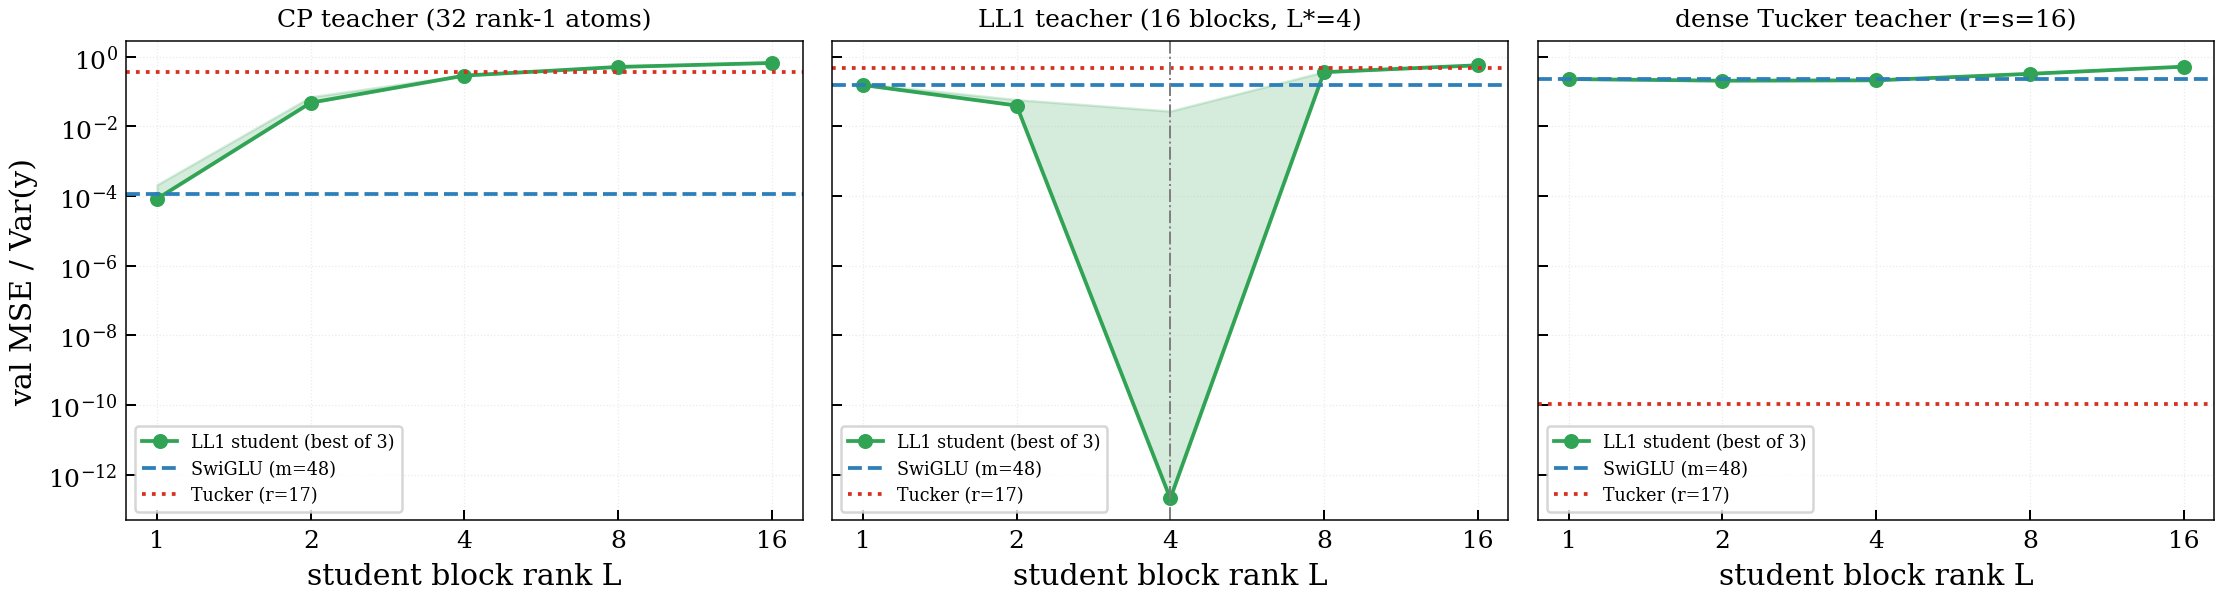
\includegraphics[width=\textwidth]{figures/exp18_lsweep.png}
\caption{Synthetic teacher--student recovery at a fixed 9{,}216-parameter student
budget ($d{=}64$; 3 seeds; line = best seed, band = seed range; log--log). Left: a CP
teacher (32 routes) is recovered by rank-one students and degrades monotonically with
student block rank $L$ as gate-tying starves routes. Middle: an LL1 teacher
($16$ blocks, $L^*{=}4$) is recovered to machine precision exactly at $L{=}4$
(dash-dot vertical line) and fails in both directions --- too few atoms below, too
few routes above. Right: a generic dense-Tucker teacher is recovered only by the
Tucker student (red dotted line at $10^{-10}$). Matched structure wins everywhere.}
\label{fig:synthetic}
\end{figure}

\subsection{Compressing real FFN maps: pretrained layers prefer small $L > 1$}
\label{sec:distill}

\textbf{Question.} Which tensor structure best describes the input--output function a
\emph{real, pretrained} SwiGLU FFN computes?

\textbf{Setup.} We capture FFN inputs and outputs for layers $\{4, 12, 20\}$ of
Qwen2.5-0.5B ($d{=}896$, $m{=}4864$; 13.07M parameters per FFN) on $\approx$120K
tokens of FineWeb-Edu, and fit students of every family at compression budgets
$\{0.6, 1.2, 2.4\}$M parameters ($4.6$--$18.4\%$ of the teacher) by MSE. 2 seeds; the
seed spread is $\pm 0.001$ rel.\ MSE throughout, so all reported gaps are
$\gtrsim 30\times$ noise.

\textbf{Result.} The ordering
$\text{LL1}(L{\approx}4\text{--}16) < \text{LL1}(2) < \text{CP} \ll \text{dense
Tucker}$ holds in all nine (layer, budget) cells (Figure~\ref{fig:distill}). LL1's
gain over CP is modest but systematic (2--4\% rel.\ MSE; e.g.\ layer 12 at 2.4M:
$0.348$ vs $0.361$), with a shallow optimum at $L \approx 4$--$8$. The $L{=}1$
control matches SwiGLU to $\pm 0.001$ in every cell. Dense Tucker is worse by
35--130\% rel.\ MSE and does not improve --- on layer 20 it \emph{worsens} --- with
budget.

\textbf{Interpretation.} The function computed by a trained SwiGLU layer contains
cross-atom structure that rank-one routed atoms capture inefficiently: at matched
budget, spending parameters on rank-4--8 routed blocks (and accepting
$3{-}10\times$ fewer routes) is consistently the better trade. The dense core is the
wrong basis for this function class at compression budgets.

\textbf{Caveat.} This is the compression regime; it measures the structure of the
teacher's function, not end-to-end trainability (next subsection). One model family
(Qwen2.5) and one dataset.

\begin{figure}[t]
\centering
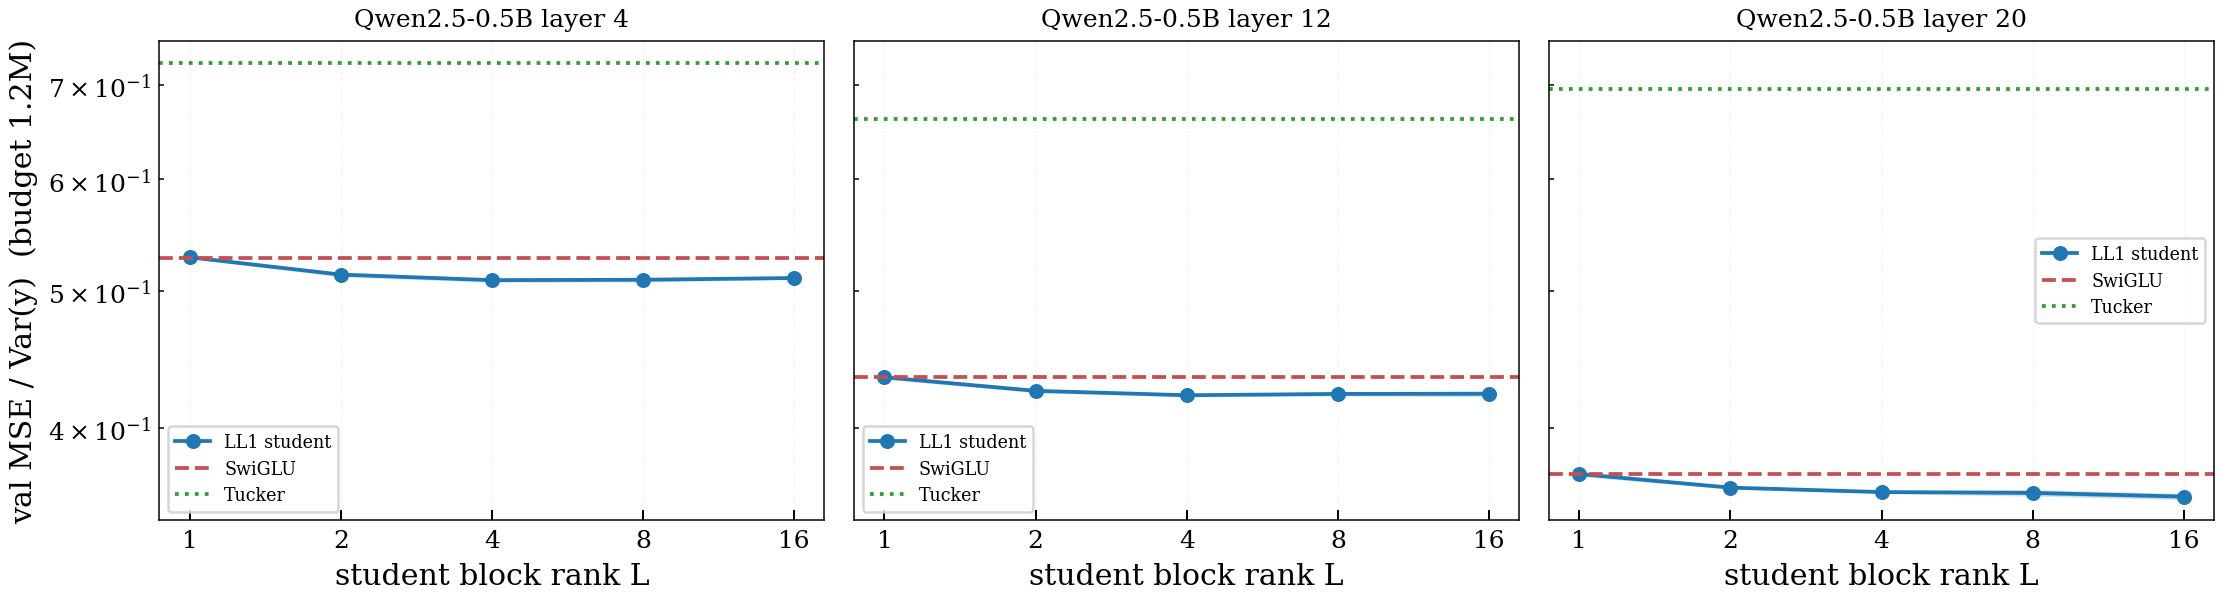
\includegraphics[width=\textwidth]{figures/exp21_distill.png}
\caption{Distilling pretrained Qwen2.5-0.5B FFN layers into matched-budget students
(relative validation MSE at the 1.2M-parameter budget; 2 seeds, spread $\pm0.001$;
log--log). In every layer the LL1 student improves on the SwiGLU/CP student
(dashed blue) with a shallow optimum at block rank $L\approx4$--$16$, and the dense
Tucker student (dotted red) is far worse. Real FFN maps contain routed low-rank block
structure.}
\label{fig:distill}
\end{figure}

\subsection{Matched-budget language modeling: a three-way tie on loss; a $2\times$ split on speed}
\label{sec:lm}

\textbf{Question.} Do these representational differences survive end-to-end training
on language?

\textbf{Setup.} LLaMA-style decoders (52.5M parameters, $d{=}512$, 8 layers) trained
from scratch on 100M FineWeb-Edu tokens with identical hyperparameters, differing
only in FFN (Table~\ref{tab:configs}); 3 seeds for SwiGLU, LL1($L{=}4$), and Tucker;
1 seed for the remaining $L$ values. Tucker uses its best-known (diagonal warm-start)
initialization. Throughput is measured separately on an idle A40.

\textbf{Result.} Final validation loss: LL1($L{=}4$) $4.7472 \pm 0.0041$, SwiGLU
$4.7542 \pm 0.0104$, Tucker $4.7626 \pm 0.0071$ (mean $\pm$ std over 3 seeds;
Figure~\ref{fig:lm}). LL1 vs.\ SwiGLU is a statistical tie (Welch $t \approx 1.1$);
LL1 vs.\ Tucker separates ($t \approx 3.1$). The $L$-sweep is flat with a shallow
optimum away from the corners (single seeds: $L{=}1$: $4.765$ --- matching SwiGLU's
range and confirming the $L{=}1\equiv$SwiGLU control end-to-end; $L{=}2$: $4.740$;
$L{=}8$: $4.742$; $L{=}16$: $4.750$). Training throughput at matched FLOPs
($4.59{\times}10^6$ MACs/token/layer for every architecture): LL1 75.3K tokens/s,
SwiGLU 71.4K, Tucker 36.5K --- LL1 is $5$--$7\%$ faster than SwiGLU (its gate
projection is a factor $\tfrac{2L+1}{3}$ narrower, and the gating multiply touches
$B$ rather than $m$ columns) and $2.06\times$ faster than Tucker, whose core
contraction is GEMM-unfriendly.

\textbf{Interpretation.} At this scale the route/atom trade is loss-neutral on
language modeling: tripling per-route rank while tripling down on routes neither
helps nor hurts. The differences that survive are operational: LL1 buys a throughput
edge and a structurally bounded per-route rank at zero loss cost, while the dense
core costs $2\times$ wall-clock for nominally identical FLOPs and slightly worse
loss.

\textbf{Caveat.} 52.5M parameters, 100M tokens, one dataset, hyperparameters
inherited from SwiGLU tuning; the $L$-sweep is single-seed away from $L{=}4$.

\begin{figure}[t]
\centering
\begin{minipage}{0.48\textwidth}
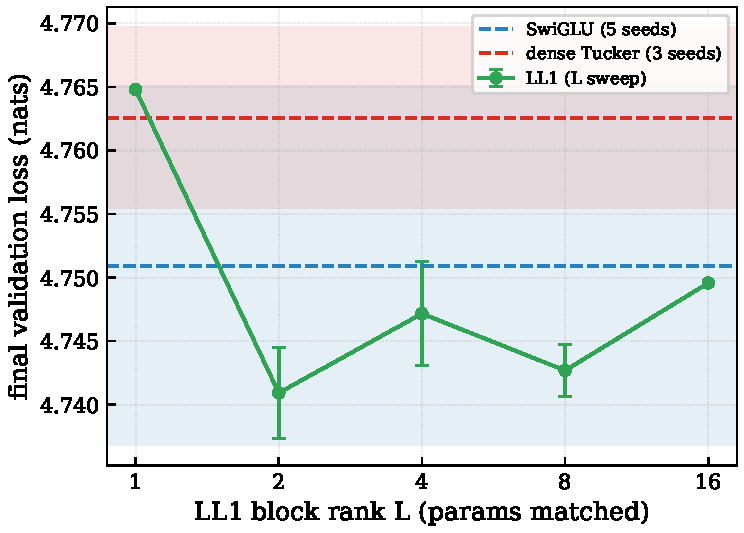
\includegraphics[width=\textwidth]{figures/lm_lsweep.pdf}
\end{minipage}\hfill
\begin{minipage}{0.50\textwidth}

\includegraphics[width=\textwidth]{figures/lm_curves.pdf}
\end{minipage}
\caption{Matched-budget language modeling (52.5M parameters, 100M FineWeb-Edu
tokens). Left: final validation loss across the LL1 block-rank sweep (error bar =
std over 3 seeds at $L{=}4$; other $L$ single-seed), with SwiGLU (blue) and dense
Tucker (red) 3-seed bands. Every $L \ge 2$ sits at or below the SwiGLU mean; the
sweep is flat. Right: validation-loss curves (mean $\pm$ std over 3 seeds) ---
the three families are indistinguishable through training.}
\label{fig:lm}
\end{figure}

\subsection{Interpretability proxies: the computation has rank $\approx 4$ per route, and no architecture routes sparsely}
\label{sec:interp}

\textbf{Question.} What does block rank buy or cost in measurable structure?

\textbf{Setup.} On the trained LMs: per-token unit contributions and their
exp-entropy (``effective active units''), all-layer top-$k$ decomposition curves,
single-unit ablations, weight-based per-gate stable ranks, and cross-seed factor
matching with shuffled-weight nulls (Appendix~\ref{app:details}).

\textbf{Result.} (i) The trained dense Tucker models use per-gate stable rank
$3.97/3.99/3.97$ (three seeds; max 5.3) of an available 128; LL1's realized rank
tracks but under-saturates its cap ($1.83$ at $L{=}2$, $3.26$ at $L{=}4$, $5.62$ at
$L{=}8$). With the distillation knee at $L \approx 4$--$8$, three independent
measurements give the same answer: \emph{the natural per-route rank of FFN
computation at this scale is $\approx 4$--$6$}. (ii) No architecture routes sparsely:
effective active units per token are 49\% of capacity for SwiGLU (733/1493), 63\% for
LL1 (312/498), 64\% for Tucker (82/128); to stay within 0.03 nats of base loss,
SwiGLU needs $\sim$34\% of its atoms per token, LL1 $\sim$51\% of blocks, Tucker
$\sim$100\% of gates (Figure~\ref{fig:interp}). (iii) Single-unit ablations are
negligible for all (max $\Delta$loss $\le 0.0016$ nats). (iv) Cross-seed recurrence:
SwiGLU's joint atoms match across seeds at $3.0\times$ the shuffled null (cosine
0.268 vs.\ 0.089); gauge-invariant per-route matrices recur weakly for SwiGLU
($1.7\times$ null) and Tucker ($1.6\times$) but are \emph{at chance for LL1}; gate
directions are at chance for every architecture.

\textbf{Interpretation.} The rank-4 convergence is the cleanest structural fact this
sprint produced, and it argues for LL1 as the \emph{honest parameterization}: it
hard-codes the rank the unconstrained model learns anyway, at lower cost. But the
interpretability proxies do not support the hypothesis that this buys mechanistic
legibility: routing stays diffuse, blocks are individually dispensable, and LL1's
learned blocks recur across seeds no better than chance --- the block partition
apparently adds assignment freedom that atom-level CP does not have.

\textbf{Caveat.} Proxies measure routing statistics and weight structure, not
semantic legibility; no human or automated interpretation of atoms/blocks was
attempted. The Tucker stable-rank value is conditional on the diagonal warm-start
initialization (the only one that reaches SwiGLU-level loss; prior work on this
codebase found random-init Tucker converges to stable rank $\approx 27$ at worse
loss); the distillation knee and the LL1 cap-saturation pattern are
initialization-independent corroborations.

\begin{figure}[t]
\centering
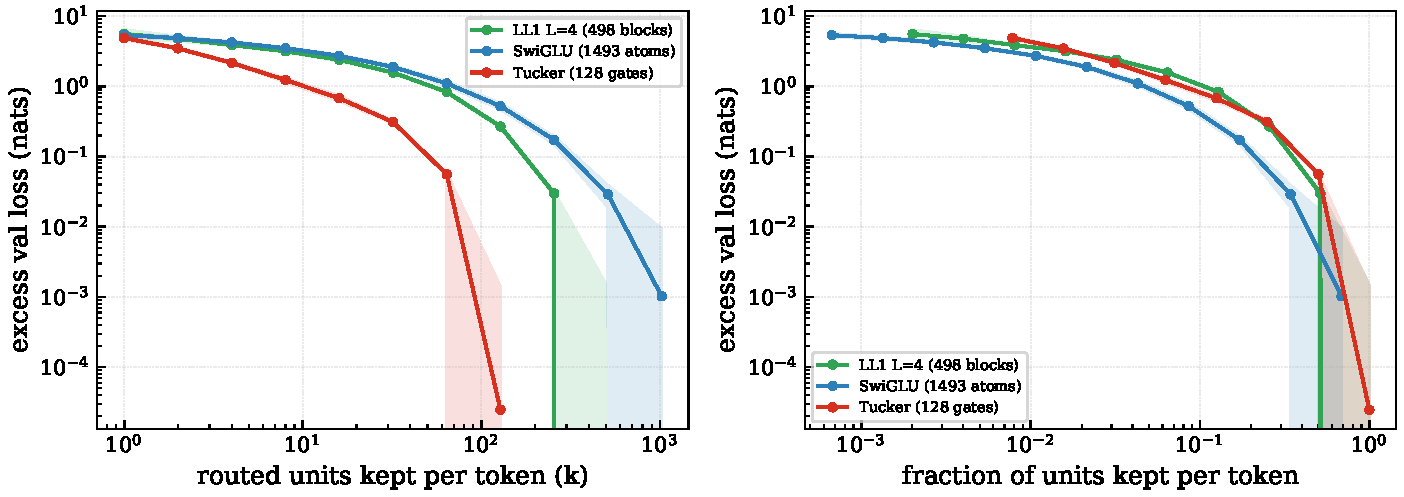
\includegraphics[width=\textwidth]{figures/interp_topk.pdf}
\caption{Top-$k$ decomposability of the trained LMs: excess validation loss when
every layer's FFN output is replaced by its $k$ largest-contribution routed units per
token (left: absolute $k$; right: fraction of available units; mean over 3 seeds for
SwiGLU/LL1, 2--3 for Tucker; log--log). SwiGLU is the most truncatable relative to
capacity, Tucker the least; LL1 sits between, with $3\times$ fewer (larger) objects
than SwiGLU at equal excess loss.}
\label{fig:interp}
\end{figure}

\subsection{Circuit pilot: induction emerges identically; one dense-core seed finds another circuit}
\label{sec:induction}

\textbf{Question.} Does FFN tensor structure change the emergence or mechanism of a
known attention circuit?

\textbf{Setup.} Repeated-sequence induction task ($[s;s]$, fresh random $s$ each
sample, vocab 128, $|s|{=}64$); 2-layer transformers ($d{=}128$) identical except
the FFN (matched 131K-parameter budgets; attention-only control); 3 seeds; we track
second-half accuracy, the canonical induction score (attention mass at offset
$|s|{-}1$), attention-offset profiles, and head/FFN ablations.

\textbf{Result.} Emergence is architecture-independent: every FFN variant reaches
$100\%$ accuracy in 140--180 steps (attention-only: 80). All SwiGLU/LL1 runs and 2/3
Tucker runs converge to textbook induction attention (offset-$63$ mass
$0.93$--$1.00$). One Tucker seed reaches $100\%$ accuracy with \emph{no} canonical
induction head: its layer-2 heads attend at diffuse offsets (mass $\le 0.19$ spread
over offsets 37--56), ablating its best head changes nothing, and its solution runs
through the FFN. A methodological caution: zeroing all FFNs collapses \emph{every}
architecture (including SwiGLU, to 13\%), so FFN-bypass is not a valid
circuit-attribution test for jointly trained models; the offset profiles are the
discriminating measurement.

\textbf{Interpretation.} A negative result for the hypothesis that FFN tensor
structure modulates circuit emergence at this scale, plus a single-seed existence
proof that the dense-core FFN admits a qualitatively different copying
implementation. We report the latter as an observation ($n{=}1$ of 3 seeds), not a
claim about frequency.

\textbf{Caveat.} Tiny models, one task, three seeds; the alternative-circuit
observation needs a basin-frequency study.

\section{Discussion}
\label{sec:discussion}

\paragraph{What is established.}
Per-route interaction rank is a real capacity dial: at fixed parameters it binds in
both directions in controlled recovery, and three independent measurements --- the
learned stable rank of an unconstrained Tucker core ($\approx 3.98$, replicated), the
saturated rank of capped LL1 blocks ($3.26$ of 4), and the compression optimum on
pretrained FFN maps ($L \approx 4$--$8$) --- agree that LM FFN computation at this
scale uses rank $\approx 4$ per route. Given that, the dense Tucker core is a
dominated design point: it spends $91\%$ of its budget parameterizing interactions it
will not use, costs $2\times$ wall-clock at matched FLOPs, and ends nominally last on
validation loss. The structured middle of the family is free: LL1 at $L{=}4$ matches
SwiGLU's loss with a small throughput edge while fixing, by construction, the rank
structure the unconstrained model discovers by itself.

\paragraph{What is plausible but not established.}
That LL1's advantages grow with scale (its compression edge on real maps suggests the
function class is right, but 52.5M-parameter training cannot confirm it); that the
route/atom trade has a scale- or data-dependent optimum away from $L{=}1$--$4$; that
rank-4 blocks are semantically coherent objects.

\paragraph{What failed.}
Our pre-registered interpretability hypothesis --- that LL1 would land between SwiGLU
and Tucker on diffuseness while keeping CP-like factor stability --- is unsupported.
Routing is diffuse for every architecture (49--64\% of capacity effectively active
per token); and on the one proxy where architectures separate, cross-seed factor
recurrence, LL1 is the only family \emph{at chance} under a gauge-invariant test that
SwiGLU and Tucker both pass weakly. Identifiability of a decomposition given a fixed
function evidently does not imply stability of the learned function's factors across
training runs. The circuit pilot returned a clean null on emergence.

\paragraph{Limitations.}
One scale (52.5M / 100M tokens), one dataset and tokenizer, hyperparameters inherited
from SwiGLU tuning (no per-architecture tuning; this likely flatters the baseline),
Tucker evaluated with its best-known initialization and weight-decay exemption on the
core (an asymmetry in its favor), single-seed $L$-sweep away from $L{=}4$,
compression-regime distillation only, and statistical interpretability proxies rather
than semantic evaluation of learned blocks.

\paragraph{Next step.}
The single most informative follow-up is a 10$\times$-scale repeat of the $L$-sweep
(${\ge}300$M parameters, ${\ge}1$B tokens, per-architecture learning-rate tuning,
${\ge}3$ seeds) testing whether the rank-4 optimum, the loss tie, and the throughput
edge persist; second, a trained sparse variant (L1 on block routes) targeting the
routing diffuseness that post-hoc truncation cannot remove.

\section{Related work}
\label{sec:related}

\paragraph{Gated FFNs and bilinear MLPs.}
GLU-family FFNs outperform ReLU/GELU MLPs at matched scale and are standard in modern
LMs \citep{shazeer2020glu}. \citet{pearce2025bilinear} study bilinear MLPs --- GLUs
with the element-wise nonlinearity removed --- which are exactly third-order tensors,
and show that eigendecomposition of those tensors yields interpretable low-rank
structure; \citet{dooms2024case} make the architectural case. Our object differs in
keeping the gate: SwiGLU is exactly a \emph{routed} CP tensor field whose routing is
input-dependent, and prior experiments on this codebase show the routing is
load-bearing (constant-$\alpha$ ablations degrade pretrained Qwen models by four to
six orders of magnitude in perplexity), so the bilinear picture alone does not
describe trained SwiGLU models. \citet{jayakumar2020multiplicative} situate gating
within multiplicative interactions broadly; we study the specific tensor
decompositions a gated FFN admits.

\paragraph{Tensor decompositions in neural networks.}
CP, Tucker, and block-term decompositions are classical
\citep{kolda2009tensor,delathauwer2008blockterm}. In deep learning they are most
often used for \emph{compression} of trained weights \citep{novikov2015tensorizing}
or for expressivity analyses of idealized architectures \citep{cohen2016expressive};
factorization machines use low-rank multiplicative atoms for feature interactions
\citep{rendle2010factorization}; \citet{loconte2024relationship} connect tensor
factorizations to probabilistic circuits. Our use is different: the decomposition is
not applied post hoc to a weight tensor --- the FFN \emph{is} the decomposition, and
we ask which member of the CP$\to$LL1$\to$Tucker family is the right parameterization
to train.

\paragraph{Sparse dictionaries and weight-based interpretability.}
Sparse autoencoders and transcoders decompose activations into feature directions
\citep{bricken2023monosemanticity,dunefsky2024transcoders,paulo2025transcoders}.
The routed-CP/LL1 view is complementary: atoms and routes are \emph{architectural}
objects fixed in the weights, with the input-dependence isolated in scalar routing
coefficients --- the same invariant-dictionary + input-dependent-coefficients
factorization transcoders recover empirically.

\paragraph{Structured matrices for efficiency.}
Monarch and butterfly factorizations replace dense projections with products of
block-diagonal or sparse factors \citep{dao2022monarch,dao2019butterfly}; LoRA
demonstrates that rank constraints are effective in transformers \citep{hu2022lora}.
These address the \emph{factor matrices}; our axis is the \emph{latent core}
connecting them. The two are orthogonal and composable.

\paragraph{Circuit-level evaluation.}
Induction heads are the canonical recognizable circuit
\citep{elhage2021mathematical,olsson2022context}; we use a minimal induction task to
ask whether FFN tensor structure changes the emergence or mechanism of an
attention-side circuit.

\bibliographystyle{plainnat}
\bibliography{refs}

\appendix

\section{The aligned-width theorem}
\label{app:theorem}

This appendix restates, with proof, the separation theorem from the earlier draft
accompanying this codebase, and records its constructive half as the LL1
architecture. Throughout, $\phi = \silu$; the only properties used are $\phi(0)=0$
and $\phi(1) \ne 0$.

\begin{lemma}[SwiGLU recovery]
\label{lem:recovery}
Setting $r=s=m$, $P=W$, $Q=G$, $R=U\T$, and $C_{oij} = \delta_{oi}\delta_{ij}$ in
\eqref{eq:tuckerffn} reduces the Tucker-core FFN to the SwiGLU map \eqref{eq:swiglu}.
\end{lemma}

\begin{proof}
With the superdiagonal core, \eqref{eq:tuckerffn} collapses to
$z_o = p_o\,\phi(q_o)$, so $z = (P\T x) \odot \phi(Q\T x)$, which is $h$ from
\eqref{eq:swiglu}; then $y = Rz = U\T h$.
\end{proof}

\begin{definition}[Aligned SwiGLU representation]
\label{def:aligned}
Given latent matrices $P, Q \in \R^{d\times r}$, an \emph{aligned width-$m$ SwiGLU
representation} is a map
\[
\hat y(x) = \sum_{j=1}^{r} \sum_{\nu=1}^{k_j} u_{j\nu}\, (a_{j\nu}\T p)\,\phi(q_j),
\qquad \textstyle\sum_j k_j = m,
\]
with $u_{j\nu} \in \R^d$, $a_{j\nu} \in \R^r$, $p = P\T x$, $q = Q\T x$. Each unit
uses a main vector in $\mathrm{span}(P)$ and one of the gate vectors $Q_{:j}$.
\end{definition}

\begin{theorem}[Diagonal bottleneck]
\label{thm:bottleneck}
Assume $[P\;Q] \in \R^{d\times 2r}$ has full column rank. The minimum width of an
aligned SwiGLU representation exactly realizing a Tucker-core FFN with per-gate
coefficient matrices $\{V_j\}_{j=1}^r$ is $m_{\min} = \sum_{j=1}^{r} \rank V_j$.
\end{theorem}

\begin{proof}
\emph{Lower bound.} By the rank assumption, $x \mapsto (p, q)$ is surjective onto
$\R^r \times \R^r$, so an exact representation forces
$\sum_j (V_j - \hat V_j)\, p\, \phi(q_j) = 0$ for all $(p,q)$, where
$\hat V_j = \sum_\nu u_{j\nu} a_{j\nu}\T$ has rank at most $k_j$. Fix $j_0$ and set
$q_j = \delta_{jj_0}$; since $\phi(0) = 0$ and $\phi(1) \ne 0$, only the $j_0$ term
survives and $V_{j_0} = \hat V_{j_0}$. Hence $k_j \ge \rank V_j$ for every $j$, and
$m = \sum_j k_j \ge \sum_j \rank V_j$.

\emph{Tightness.} Let $V_j = \sum_{\nu=1}^{\rho_j} u_{j\nu} a_{j\nu}\T$ be any rank
decomposition, $\rho_j = \rank V_j$. Then
$V_j\, p\, \phi(q_j) = \sum_\nu u_{j\nu} \big((P a_{j\nu})\T x\big)\,
\phi(Q_{:j}\T x)$ is a sum of $\rho_j$ aligned units sharing gate $Q_{:j}$.
\end{proof}

\begin{corollary}[Generic separation]
If $R$ has full column rank and each slice $C^{(j)}$ is generic, then
$\rank V_j = \min(r,s)$ for all $j$ and $m_{\min} = r \min(r,s)$; in the balanced
case $r=s=k$, $m_{\min} = k^2$.
\end{corollary}

\begin{remark}[The constructive half is LL1]
The tightness construction --- $\rho_j$ rank-one units sharing the gate $Q_{:j}$ ---
is precisely one block of the LL1 FFN \eqref{eq:ll1} with $L = \rho_j$. Theorem
\ref{thm:bottleneck} therefore does not say ``dense cores beat SwiGLU''; it says the
cost of simulating a routed tensor map is the sum of its per-route ranks, and an
architecture that fixes those ranks directly realizes the map at exactly that cost.
\end{remark}

\section{Experimental details}
\label{app:details}

\paragraph{Hardware.} All sprint experiments ran on two NVIDIA A40 GPUs (46\,GB).

\paragraph{Synthetic teacher--student (\S\ref{sec:synthetic}).}
$d=64$; teachers: CP $=$ LL1$(B{=}32, L{=}1)$, LL1$(B{=}16, L{=}4)$, dense Tucker
$r{=}s{=}16$ with slices resampled to full rank and core scaled by $1/r$; all factor
entries i.i.d.\ $\mathcal N(0, 1/d)$; teacher outputs normalized to unit std. Students
trained on 50{,}000 / validated on 8{,}000 inputs $x\sim\mathcal N(0, I_d)$; Adam,
lr $3{\times}10^{-3}$ cosine-annealed to 1\%, batch 512, 5{,}000 steps, 3 seeds per
cell. Budgets: $L$-sweep at $N{=}9216$ (within 8\% for all archs; exact counts
reported with results); budget sweep $\{0.25, 0.5, 1, 2\}{\times}N$.

\paragraph{Language modeling (\S\ref{sec:lm}).}
LLaMA-style decoder: $d{=}512$, 8 layers, 8 heads, RoPE, RMSNorm, tied embeddings,
GPT-2 BPE (50{,}257), context 1024. FFN budget matched to SwiGLU $m{=}1493$
($2.293$M/layer $\pm 0.2\%$): Tucker $r{=}s{=}128$; LL1 $(L,B) \in
\{(1,1493),(2,896),(4,498),(8,263),(16,136)\}$. AdamW $(\beta_1,\beta_2)=(0.9,0.95)$,
weight decay 0.1 (Tucker core 0.0, inherited from prior work), peak lr
$3{\times}10^{-4}$, 200-step warmup, cosine to 10\%, grad clip 1.0, batch
$24\times1024$ tokens, bf16 autocast, 100M FineWeb-Edu (sample-10BT) tokens
($\approx$4070 steps), validation on a held-out 128-sequence (131K-token) split with
deterministic seed. Tucker uses the variance-preserving diagonal warm start
($C_{ooo}{=}1$, off-diagonal std $10^{-2}/r$), the only initialization that matched
SwiGLU in prior work on this codebase. Seeds 0--2 for SwiGLU, Tucker, LL1$(L{=}4)$;
seed 0 for the remaining $L$ values.

\paragraph{Pretrained-layer distillation (\S\ref{sec:interp}).}
Teacher: Qwen2.5-0.5B \citep{yang2024qwen25} ($d{=}896$, $m{=}4864$, 13.07M
params/FFN). We capture FFN input/output pairs on $\approx$120K tokens of FineWeb-Edu
for layers $\{4, 12, 20\}$, normalize outputs to unit std, and fit students at
budgets $\{0.6, 1.2, 2.4\}$M parameters ($4.6$--$18.4\%$ of the teacher layer) by
MSE; Adam lr $2{\times}10^{-3}$, 4{,}000 steps, batch 512, 2 seeds; 90/10
train/val split.

\paragraph{Induction pilot (\S\ref{sec:induction}).}
Sequences $[s;s]$, $s$ uniform over vocab 128, $|s|=64$; 2-layer transformers,
$d{=}128$, 4 heads; FFN budget 131{,}072 params (SwiGLU $m{=}341$; LL1
$L\in\{1,4,16\}$; Tucker $r{=}48$; attention-only control). AdamW lr $10^{-3}$,
weight decay 0.01, batch 128, 3{,}000 steps, 3 seeds. Induction score: mean
attention mass from second-half queries at offset $|s|-1$, max over layer-2 heads,
on a fixed 256-sequence eval batch.

\paragraph{Interpretability proxies (\S\ref{sec:interp}).}
Contributions computed on 4096 randomly sampled token positions from a held-out
32-sequence validation set. Unit contributions: SwiGLU $c_j = |h_j|\,\|u_j\|$;
LL1 $c_b = \|U_b r_b\|\,|\silu(g_b\T x)|$; Tucker $c_j = \|V_j p\|\,|\silu(q_j)|$.
Top-$k$ curves replace every layer's FFN output by the sum of its $k$
largest-contribution units per token. Single-unit ablations zero one atom (SwiGLU),
one block-gate (LL1), or one latent gate (Tucker; $\silu(0)=0$ removes the slice
exactly) in one layer and re-evaluate full-model validation loss.

\section{Additional results}
\label{app:extra}

\begin{figure}[h]
\centering
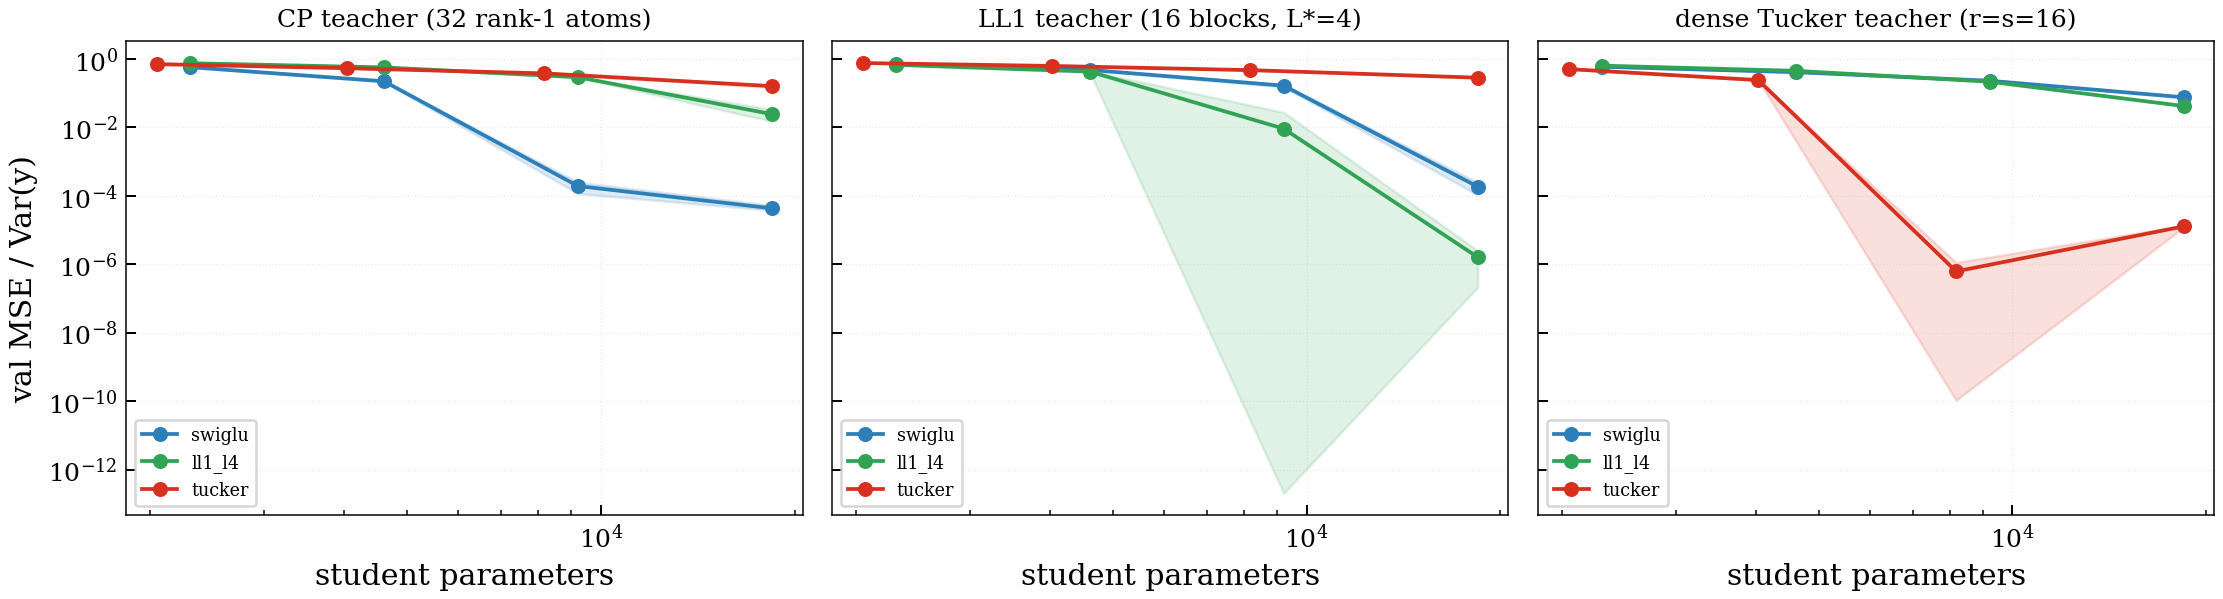
\includegraphics[width=\textwidth]{figures/exp18_budget.png}
\caption{Synthetic recovery across student parameter budgets
$\{0.25, 0.5, 1, 2\}\times 9216$ (mean over 3 seeds, band = seed range). The
matched-structure advantage of Figure~\ref{fig:synthetic} persists at every budget;
the dense Tucker student improves on non-Tucker teachers only marginally with budget
because added parameters go into its core rather than into routes.}
\label{fig:budget}
\end{figure}

\begin{figure}[h]
\centering
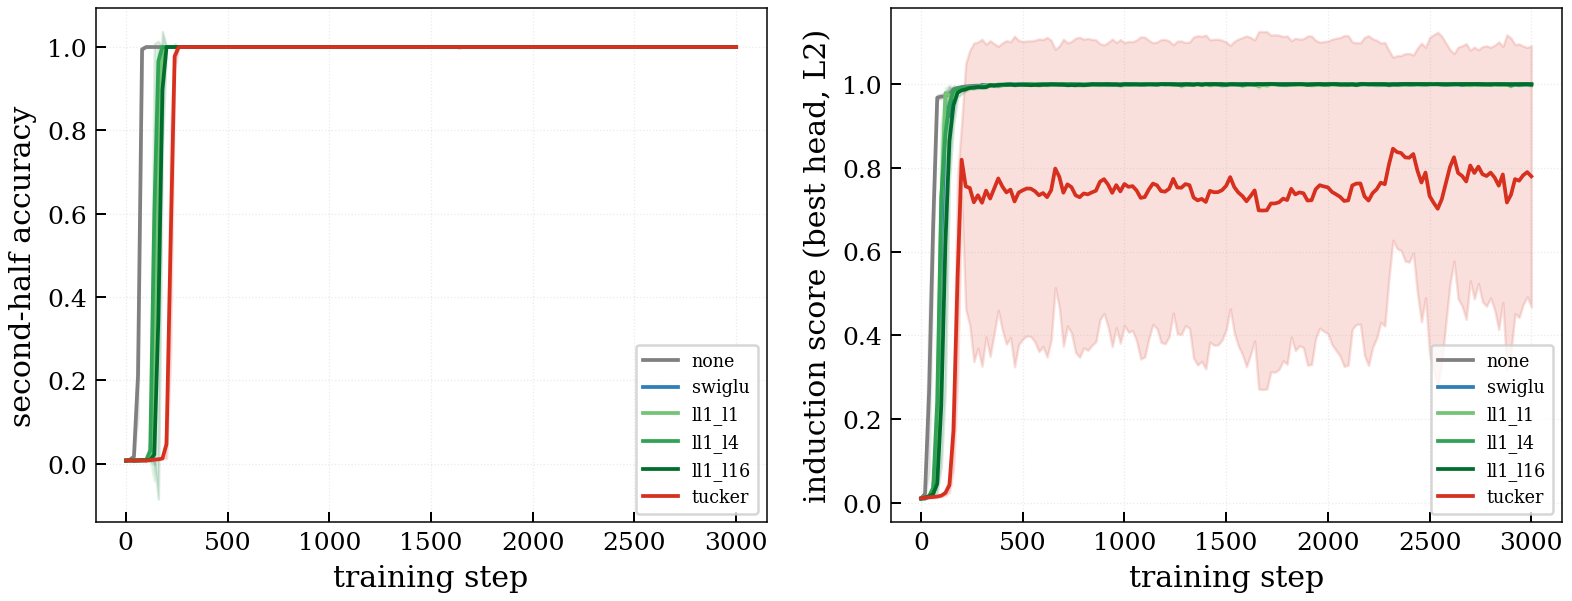
\includegraphics[width=0.85\textwidth]{figures/exp20_curves.png}
\caption{Induction pilot: second-half accuracy (left) and canonical induction score
(right) versus training step (mean $\pm$ std over 3 seeds per architecture). All FFN
variants learn the task at indistinguishable speed; the attention-only control is
faster. The Tucker induction-score band is wide because one of its three seeds
solves the task without the canonical attention pattern.}
\label{fig:induction}
\end{figure}

\begin{figure}[h]
\centering
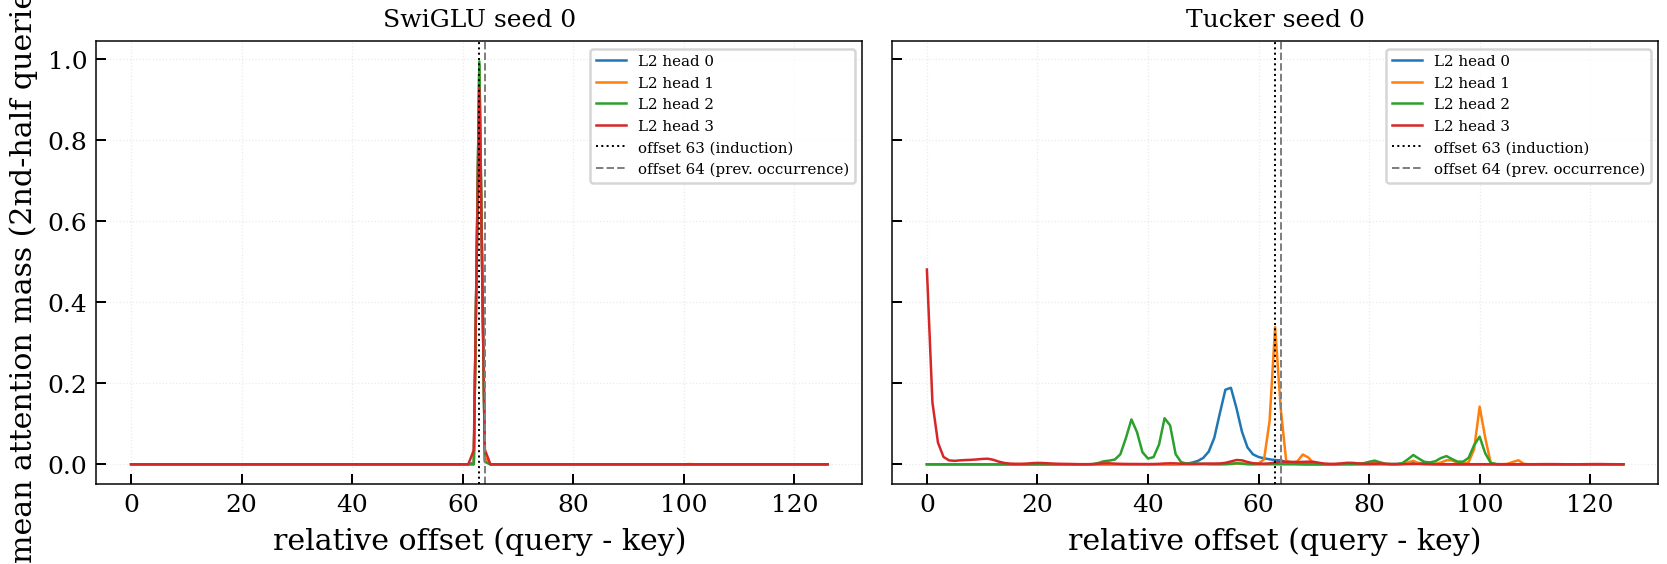
\includegraphics[width=0.95\textwidth]{figures/exp20b_offsets.png}
\caption{Layer-2 attention-offset profiles (mean attention mass from second-half
query positions to each relative offset). Left: a representative SwiGLU run --- all
heads concentrate on the canonical induction offset $|s|-1 = 63$ (mass
$0.93$--$1.0$). Right: the anomalous Tucker seed --- attention is spread over
non-canonical offsets (mass $\le 0.19$ per head), yet the model reaches $100\%$
accuracy; ablating its best head changes nothing.}
\label{fig:offsets}
\end{figure}

\end{document}
